\documentclass{beamer}

\usepackage[utf8]{inputenc}
%\usepackage[T1]{fontenc}

\usepackage{xcolor}
\usepackage{graphicx}
\usepackage{enumitem}

\usepackage{amsmath}
\usepackage{amssymb}
\usepackage{amsthm}
\usepackage{bm}

\usepackage{tikz}
\usepackage{hyperref}
\usepackage{animate}

\usetheme{Dresden}
\usecolortheme{wolverine}


\title{\textbf{Poisson's equation\\
 on an L-shaped domain}}
\date{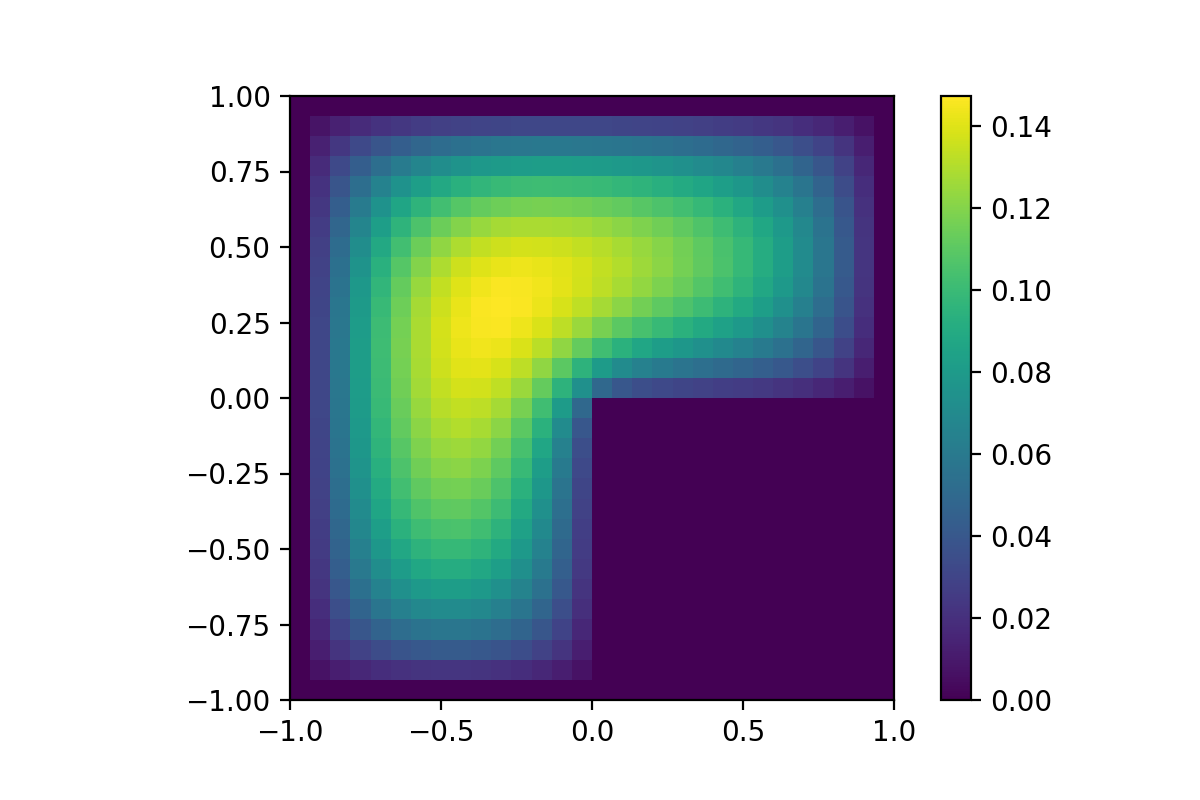
\includegraphics[width=4cm]{sol37.png}\\[2ex]
27 January 2020}
\author{Adéla Moravová \and Barbara Präg 
\vspace{-0.7cm}}


\begin{document}


\maketitle


\begin{frame}{Contents}
\tableofcontents
\end{frame}

\section{Poisson's equation}

\begin{frame}{Poisson's equation}

$\begin{cases}- \Delta u = f \ \text{in} \ \Omega  \\
\ \ \ \ \  u = 0 \ \text{on} \ \partial \Omega 
\end{cases}$\\[0.5cm]

Weak formulation with solution $u\in H_0^1(\Omega)$:\\

$\displaystyle a(u,v) = \int_\Omega \nabla u \cdot \nabla v \ \text{d}x = \int_\Omega f v \ \text{d}x = (f,v) \ \ \ \forall v \in H_0^1(\Omega)$\\[0.5cm]


\begin{minipage}[t]{0.3\textwidth}
\centering
	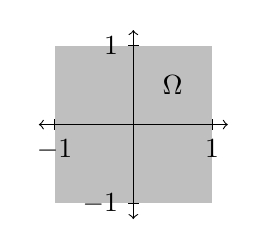
\begin{tikzpicture}[scale=1]
	%\draw (-1,-1) -- (-1,1) -- (1,1) -- (1,-1) -- (-1,-1);
 	\fill[fill = lightgray] (-1,-1) rectangle (1,1);

	\draw[<->] (-1.2,0) -- (1.2,0) coordinate (x axis);
 	\draw[<->] (0,-1.2) -- (0,1.2) coordinate (y axis);
 	
 	\foreach \x/\xtext in {-1/-1, 1/1}
 		\draw (\x,2pt) -- (\x,-2pt) node[anchor=north] {$\xtext$};
 	\foreach \y/\ytext in {-1/-1, 1/1}
 		\draw (2pt,\y) -- (-2pt,\y) node[anchor=east] {$\ytext$};
 		
 	\draw (0.5,0.5) node {$\Omega$};
 		
\end{tikzpicture}\\
\end{minipage}
\begin{minipage}[b]{0.3\textwidth}
\centering
	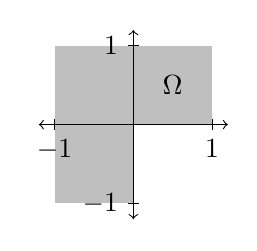
\begin{tikzpicture}[scale=1]
	%\draw (-1,-1) -- (-1,1) -- (1,1) -- (1,-1) -- (-1,-1);
 	\fill[fill = lightgray] (-1,-1) rectangle (1,1);
 	\fill[fill = white] (0,0) rectangle (1,-1);

	\draw[<->] (-1.2,0) -- (1.2,0) coordinate (x axis);
 	\draw[<->] (0,-1.2) -- (0,1.2) coordinate (y axis);
 	
 	\foreach \x/\xtext in {-1/-1, 1/1}
 		\draw (\x,2pt) -- (\x,-2pt) node[anchor=north] {$\xtext$};
 	\foreach \y/\ytext in {-1/-1, 1/1}
 		\draw (2pt,\y) -- (-2pt,\y) node[anchor=east] {$\ytext$};
 		
 	\draw (0.5,0.5) node {$\Omega$};
 		
\end{tikzpicture}
\end{minipage}
\begin{minipage}[b]{0.3\textwidth}
	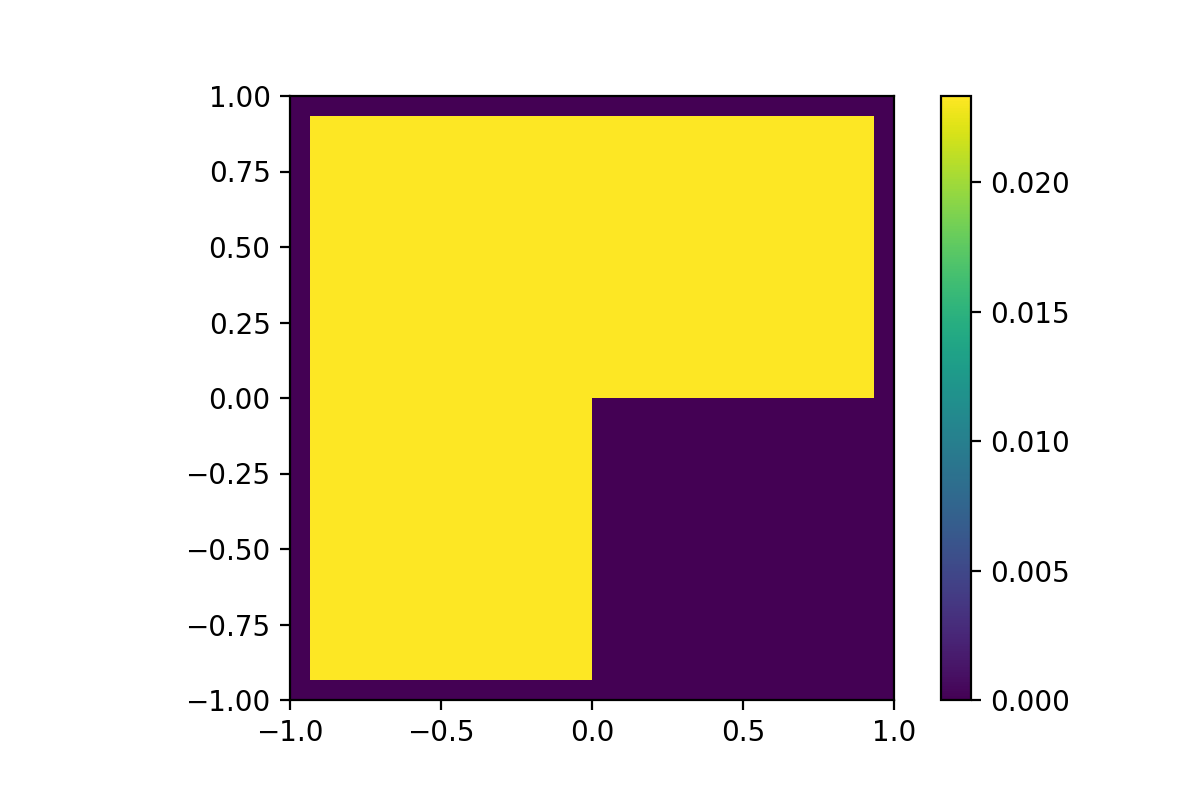
\includegraphics[height=2.6cm,trim=0 0 3.4cm 0,clip=true]{sol1.png}
\end{minipage}

\end{frame}


\begin{frame}{Reminder: Sobolev spaces and their norms}
Let $\Omega \subset \mathbb{R}^n$ be open.\\[0.8cm]

$H^k(\Omega) = \{u \in L^2(\Omega): D^\alpha u \in L^2(\Omega)$ for all $|a| \leq k\}$\\[0.5cm]
%--> $H^0(\Omega) = L^2(\Omega)$

$(u,v)_{H^k} = \sum_{|a| \leq k} \int_\Omega D^\alpha u \ D^\alpha v \ \text{d}x$\\[0.5cm]

$\|u\|_{H^k(\Omega)} = \sqrt{(u,u)_{H^k}}$\\[0.5cm]

$u \in H_0^1(\Omega)$ if $u \in H^1(\Omega)$ and "$u |_ { \partial \Omega} = 0$"
\end{frame}


\section{Shift theorems}

\begin{frame}{Shift theorems}
Let $\Omega$ be a \emph{convex polygonal} domain in $\mathbb{R}^2$ and $u$ the weak solution to our problem. Then 
\begin{equation}
	\| u \|_{H^2} \leq C \| f \|_{H^0} \ \text{for} \ f \in H^0(\Omega) = L^2(\Omega).
\end{equation}\\[0.5ex]
% --> The solution is two times more "regular" than the right-hand side f. The elliptic differential operator "smoothes"

For a smooth boundary $\partial \Omega$ it even holds that \begin{equation*}
	\|u\|_{H^{m+2}} \leq C \|f\|_{H^m} \ \text{for} \ f \in  H^m(\Omega) \ \text{and} \ m \geq 0.
\end{equation*}
%Do we need to include m=-1? Should we then define it?
%For a square $m=0$ and $m=1$ are possible.

% Similar result can be obtained for fractional-order Sobolev spaces.
% Add more here??

These regularity estimates never hold for non-convex polygonal domains like the L-shape.

\end{frame}



\begin{frame}{Numerical solution of Poisson's equation on an L-shaped domain}

regular triangulation with right-angled triangles\\
finite element method\\
conjugate gradients solver\\

\animategraphics[autoresume, height=3.5cm]{15}{sol}{1}{15}

%%% the gif but I need it in single png-frames :(
%%% Latex does apparently not accept gifs...

\end{frame}



\begin{frame}{Regularity problem of the L}

\begin{minipage}{0.4\textwidth}
\begin{tikzpicture}
    \node[anchor=south west,inner sep=0] (image) at (0,0) {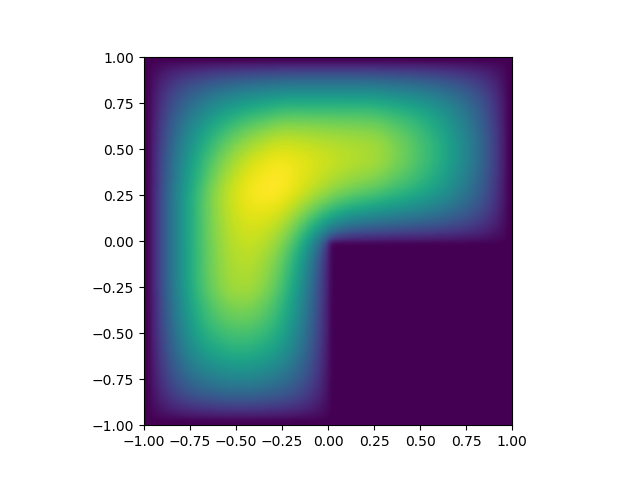
\includegraphics[height=4cm, trim=2cm 0 1.5cm 0, clip=true]{Figure_1.png}};
    \begin{scope}[x={(image.south east)},y={(image.north west)}]
    	\draw[->,red, ultra thick] (0.5,0.4845) -- (0.5,0.7);
    	\draw[->,red, ultra thick] (0.5,0.49) -- (0.3,0.49);
    	\draw[->,red, ultra thick] (0.5,0.49) -- (0.32,0.68);
        %\draw[red,ultra thick,rounded corners] (0.62,0.65) rectangle (0.78,0.75);
    \end{scope}
\end{tikzpicture}
\end{minipage}
\begin{minipage}{0.5\textwidth}
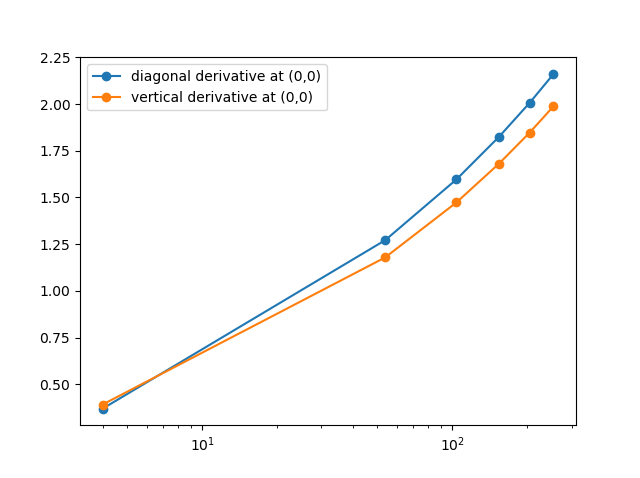
\includegraphics[height=5cm]{derivatives2.png}
\end{minipage}

\end{frame}



\section{Finite element error}

\begin{frame}{Finite element error}
Let $u$ be the weak solution of our elliptic problem, $\mathcal{T}_h$ a regular triangulation of $\Omega$ and $V_h = \{u \in C(\Omega) \cap H_0^1(\Omega): u|_T = \mathbb{P}^1 \ \forall\ T \in \mathcal{T}_h \}$ a piecewise linear finite element space.
Then for the finite element solution $u_h \in V_h$,
% i.e., $ u_h \in V_h$ such that $a(u_h,v_h) = (f,v_h)$ for all $v_h \in V_h$,
\begin{equation}
	\|u - u_h\|_{H^1(\Omega)} \leq C h \|u\|_{H^2(\Omega)}. \label{fee}
\end{equation}	
	
Under the assumption that $\Omega$ is convex and u satisfies the shift theorem (\ref{st}), we also get an $L^2$ estimation for the finite element error:\\[1ex]

\end{frame}



\begin{frame}{Finite element error}
Let $z \in H_0^1(\Omega)$ be a solution of $a(z,v) = (u-u_h,v)$ for all  $v \in H_0^1(\Omega)$.

For all $z_h \in V_h \subset H_0^1(\Omega)$, $a(u,z_h) = (f,z_h) = a(u_h,z_h)$. $\Rightarrow a(u-u_h,z_h) = 0$.\\
% $u-u_h \in H_0^1(\Omega)$, cf. \ref{fee}. and \ref{st}???

\medskip
Hence, $\|u-u_h\|_{L^2}^2 = (u-u_h,u-u_h) = a(z,u-u_h) = a(z-z_h,u-u_h) \leq$\\
$\overset{\text{CS}}{\leq} \|\nabla(u-u_h)\|_{L^2} \cdot \|\nabla(z-z_h)\|_{L^2} \leq \|u-u_h\|_{H^1}  \cdot \|z-z_h\|_{H^1} \overset{(\ref{fee})}{\leq} Ch^2 \cdot \|u\|_{H^2} \cdot \|z\|_{H^2} \leq$\\
$\overset{(\ref{st}) z}{\leq} \tilde{C}h^2\cdot \|u\|_{H^2} \cdot \|u-u_h\|_{H^0} = \tilde{C}h^2\cdot \|u\|_{H^2}\cdot \|u-u_h\|_{L^2}.$\\

\medskip
Therefore, $\|u-u_h\|_{L^2} \leq \tilde{C}h^2 \|u\|_{H^2}$.\\[2.5ex]

If $\Omega$ is not convex, this inequality need not hold true, too.\\[0.9cm]


\end{frame}

\section{Refining the grid}

\begin{frame}
Since the kink at $(0,0)$ is causing the regularity problems in the L-shape (in comparison to the square), we now refine the grid close to this critical point and compare the number of grid points we need to get a certain residual error.\\

\centering
\begin{minipage}{0.5\textwidth}
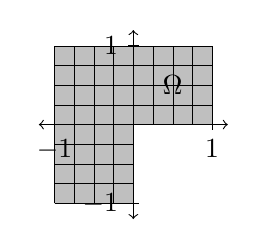
\begin{tikzpicture}[scale=1]
	%\draw (-1,-1) -- (-1,1) -- (1,1) -- (1,-1) -- (-1,-1);
 	\fill[fill = lightgray] (-1,-1) rectangle (1,1);
 	\draw[step=0.25cm, ultra thin] (-1,-1) grid (1,1);
	\fill[fill = white] (0,0) rectangle (1.1,-1.1);

	\draw[<->] (-1.2,0) -- (1.2,0) coordinate (x axis);
 	\draw[<->] (0,-1.2) -- (0,1.2) coordinate (y axis);
 	
 	\foreach \x/\xtext in {-1/-1, 1/1}
 		\draw (\x,2pt) -- (\x,-2pt) node[anchor=north] {$\xtext$};
 	\foreach \y/\ytext in {-1/-1, 1/1}
 		\draw (2pt,\y) -- (-2pt,\y) node[anchor=east] {$\ytext$};
 		
 	\draw (0.5,0.5) node {$\Omega$};
 		
\end{tikzpicture}
\end{minipage}
\begin{minipage}{0.4\textwidth}
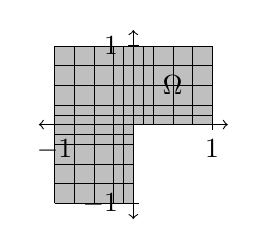
\begin{tikzpicture}[scale=1]
	%\draw (-1,-1) -- (-1,1) -- (1,1) -- (1,-1) -- (-1,-1);
 	\fill[fill = lightgray] (-1,-1) rectangle (1,1);
 	\draw[step=0.25cm, ultra thin] (-1,-1) grid (1,1);
 	\foreach \x in {0.125,-0.125}
 		\draw[ultra thin] (\x,1) -- (\x,-1);
 	\foreach \y in {0.125,-0.125}
 		\draw[ultra thin] (1,\y) -- (-1,\y);

 	\fill[fill = white] (0,0) rectangle (1.1,-1.1);

	\draw[<->] (-1.2,0) -- (1.2,0) coordinate (x axis);
 	\draw[<->] (0,-1.2) -- (0,1.2) coordinate (y axis);
 	
 	\foreach \x/\xtext in {-1/-1, 1/1}
 		\draw (\x,2pt) -- (\x,-2pt) node[anchor=north] {$\xtext$};
 	\foreach \y/\ytext in {-1/-1, 1/1}
 		\draw (2pt,\y) -- (-2pt,\y) node[anchor=east] {$\ytext$};
 		
 	\draw (0.5,0.5) node {$\Omega$};
 		
\end{tikzpicture}
\end{minipage}

\end{frame}


\begin{frame}
\vfill

\centering \Large{\textbf{Vielen Dank für eure Aufmerksamkeit!}}\\[10ex]

\begin{figure}[b!]
\normalsize
\flushleft
\vfill
\small
Literatur und Graphiken: \url{https://ocw.mit.edu/courses/
aeronautics-and-astronautics/16-07-dynamics-fall-2009/lecture-notes/MIT16_07F09_Lec30.pdf} Zugriff: \today
\end{figure}
\end{frame}



\end{document}
